
\section{Theorie}
\label{sec:Theorie}
Bei einer Linse handelt es sich um Objekt, welches sich in seiner Dichte von der seines Umgebungsmaterials unterscheidet. Das hat zu Folge, dass auf die Grenzfläche von Linse und Umgebungsmaterial treffendes Licht gebrochen wird. Linsen bestehen dabei meist aus stark Lichtdurchlässigem Material. Bei dem Umgebungsmaterial handelt es sich meistens um Luft. In diesem Versuch werden Linsen aus Glas verwendet, welche sich in einem luftgefüllten Raum befinden. In der Optik wird zwischen sogenannten \textit{Sammel}- und \textit{Zerstreuungslinsen} unterschieden. Sammellinsen laufen an den Rändern dünner zu, wodurch parallel auf die Linse treffendes Licht, beim durchtreten der Linse, auf einen Punkt, den \textit{Brennpunkt}, fokussiert wird. Dabei wird der Abstand von Linse zu Brennpunkt als \text{Brennweite} und der Abstand zwischen Linse und dem Bild der Linse als \textit{Bildweite} der Linse bezeichnet. Bildweite und Brennweite sind bei Sammellinsen positiv. Desshalb entsteht ein reelles Bild, wenn der gebrochene Lichtstrahl auf einen Bildschirm fällt. Bei Zerstreuungslinsen hingegen sind Brenn- und Bildweite negativ, wodurch ein virtuelles Bild auf dem Bildschirm entsteht. In Abbildung \ref{fig:Normal} sind alle Definitionen der behandelten Größen dargestellt. 

\begin{figure}
\begin{minipage}{0.5\textwidth}
    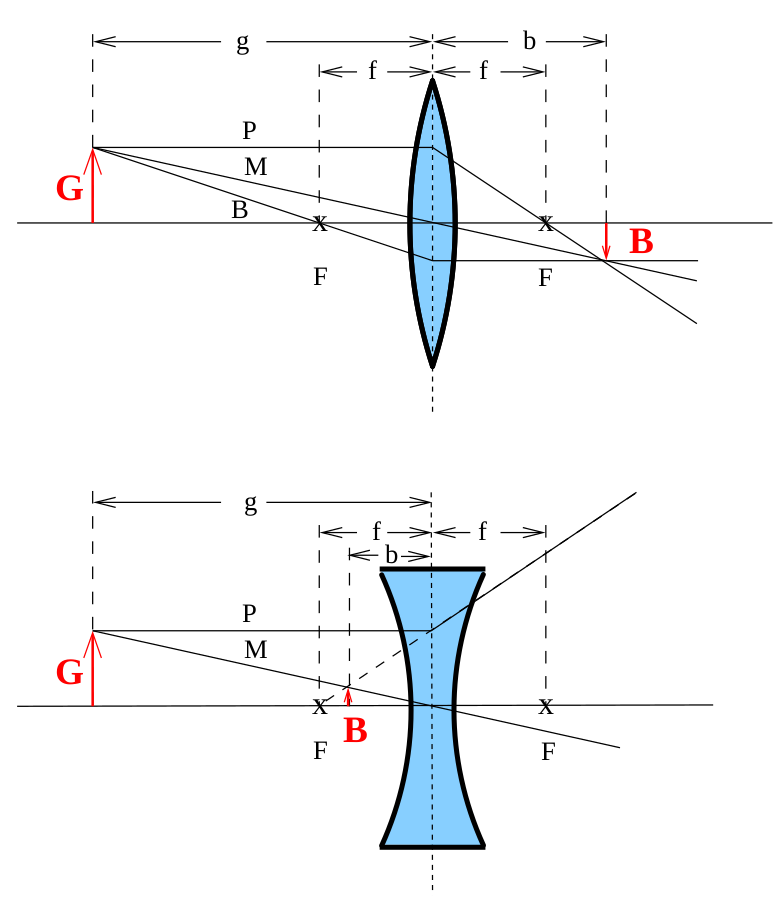
\includegraphics[width=\textwidth]{data/Normale_Linsen.png}
\end{minipage}
\begin{minipage}{0.5\textwidth}
\begin{align*}
    \text{f} & \equiv \text{Brennweite} \\
    \text{b} & \equiv \text{Bildweite} \\
    \text{g} & \equiv \text{Gegenstandsweite} \\
    \text{F} & \equiv \text{Brennpunkt} \\
    \textcolor{red}{G} & \equiv \text{Gegenstandsgröße} \\
    \textcolor{red}{B} & \equiv \text{Bildgröße} \\
    \text{P} & \equiv \text{Parallelstrahl} \\
    \text{M} & \equiv \text{Mittelpunktstrahl} \\
    \text{B} & \equiv \text{Brennpunktstrahl}
\end{align*}
\end{minipage}
\caption{Schematische Darstellung einer Sammel-(Oben) und Zerstreuungslinse (Unten) mit dazugehöriger Bildkonstruktion.}
\label{fig:Normal}
\end{figure}

Es ist zu Beachten, dass die Brechung bei diesen beiden dünnen Linsen auf die \textit{Mittelebene} reduzuiert ist. Bei dicken Linsen (Abbildung \ref{fig:Dick}) ist diese Vereinfachung nicht mehr annehmbar. Aus dem Grund werden zwei \textit{Hauptebenen} eingeführt. Anstatt nur an der Mittelebene gebrochen zu werden, wird der Lichtstrahl an beiden Hauptebenden gebrochen gedacht.

\begin{figure}
    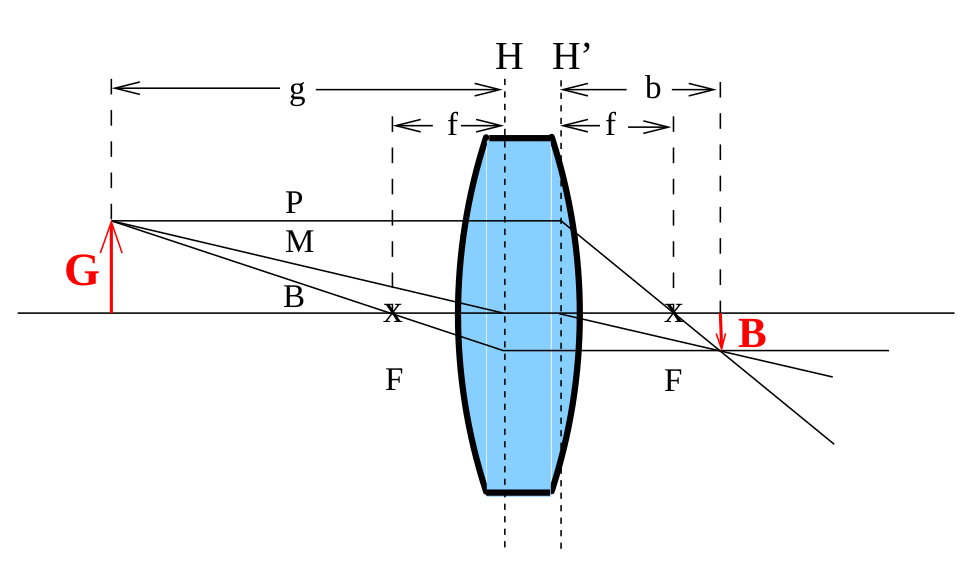
\includegraphics[width=\textwidth]{data/Breite_Linse.png}
    \caption{Bildkonstruktion bei einer dicken Sammellinse.}
    \label{fig:Dick}
\end{figure}

Bei der Bildkonstruktion werden drei ausgezeichnete Strahlen verwendet. Der Parallelstrahl, der Mittelpunktstrahl und der Brennpunktstrahl. Dabei verläuft der Parallelstrahl senkrecht zu der Mittelebene der Linse. Beim durchscheinen wird dieser Strahl auf den Brennpunkt fokussiert und wird damit zum Brennpunktstrahl. Der Mittelpunktstrahl läuft durch den Mittelpunkt der Linse und ändert dabei seine Richtung nicht. Die Definitionen sind der Abbildung \ref{fig:Normal} zu entnehmen. 

Aus den Strahlensätzen lassen sich die Verhältnisse 
\begin{equation}
    V=\frac{\textcolor{red}{B}}{\textcolor{red}{G}} = \frac{b}{g}
\end{equation}
ableiten. Dieses Verhältnis wird \textit{Abbildungsgesetz} genannt, wobei $V$ dem Abbildungsmaßstab entspricht. 
Aus diesem Gesetz lässt sich für dünne Linsen die \textit{Linsengleichung}
\begin{equation}
    \frac{1}{f}=\frac{1}{b}+\frac{1}{g}
    \label{eqn:linsengl}
\end{equation}
herleiten.
Damit die Linsengleichung auch für dicke Linsen verwendet werden kann, müssen Bildweite, Gegenstandsweite und Brennweite von der jeweiligen Hauptebenden aus definiert werden.


Die Vereinfachung, die Brechung der Linse auf die Brechung der Mittelebene zu reduzuieren, verliert bei achsenfernen Strahlen an Genauigkeit. Es treten Abbildungsfehler auf, welche sich in der Verschiebung des Brennpunkts manifestieren. Bei der spährischen Abberration liegt der Brennpunkt von achsennahen Strahlen von der Linse entfernter als die achenfernen. Ein ähnlicher Effekt tritt bei Licht unterschiedlicher Farben auf. Bei der chromatischen Abberration liegt der Brennpunkt von blauen Licht näher an der Linse als von rotem Licht. 
Ein Charakteristikum einer Linse ist die sogenannte \textit{Brechkraft}, welche über $D=\frac{1}{f}$, mit der Einheit [dpt], definiert wird. 
Wird ein Linsensystem aus Linsen mit bekannter Brechkraft zusammengesetz, so ergibt sich die Brechkraft des gesamten Linsensystems über die Summe der einzelnen Brechkräfte
\begin{equation}
    D_\text{Linsensystem}=\sum_i^N D_i .
\end{equation}






%In knapper Form sind die physikalischen Grundlagen des Versuches, des Messverfahrens, sowie sämtliche für die Auswertung erforderlichen Gleichungen darzustellen. (Keine Herleitung)

%(eventuell die Aufgaben)

%Der Versuchsaufbau: Beschreibung des Versuchs und der Funktionsweise (mit Skizze/Bild/Foto)
